\documentclass[tikz,border=3pt]{standalone}
\usepackage[utf8]{inputenc}
\usepackage[T1]{fontenc}
\usepackage{lmodern}
\renewcommand{\familydefault}{\sfdefault}
\usepackage{sansmath}\sansmath
\usepackage{chemfig}
\usepackage{pgfplots}\pgfplotsset{compat=1.18,/pgf/number format/use comma,/pgf/number format/1000 sep={.}}
\usetikzlibrary{arrows.meta,calc,positioning,decorations.pathmorphing,patterns}
% paleta del sitio
\definecolor{nar}{HTML}{E8680C}\definecolor{narc}{HTML}{FFB35C}\definecolor{hielo}{HTML}{FFF3E8}
\definecolor{tinta}{HTML}{1D1D1F}\definecolor{gris}{HTML}{6E6E73}\definecolor{lila}{HTML}{7C5CF0}
\definecolor{azul}{HTML}{2F6FD6}\definecolor{menta}{HTML}{17A673}\definecolor{coral}{HTML}{E8342A}
\begin{document}
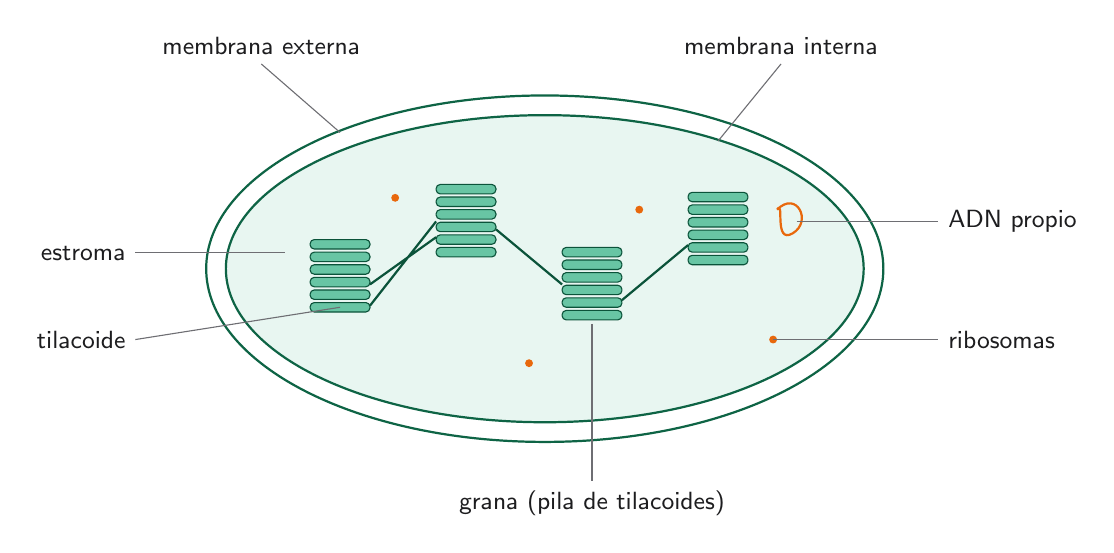
\begin{tikzpicture}[font=\small]
\draw[menta!60!black,thick,fill=white] (0,0) ellipse (4.3 and 2.2);
\draw[menta!60!black,thick,fill=menta!10] (0,0) ellipse (4.05 and 1.95);
\foreach \x/\y in {-2.6/-0.55,-1.0/0.15,0.6/-0.65,2.2/0.05}{
  \foreach \k in {0,...,5} \draw[menta!50!black,fill=menta!65,rounded corners=1.5pt] (\x-0.38,\y+\k*0.16) rectangle (\x+0.38,\y+\k*0.16+0.12);}
\draw[menta!50!black,thick] (-2.22,-0.2) -- (-1.38,0.4) (-0.62,0.5) -- (0.22,-0.2) (0.98,-0.4) -- (1.82,0.3) (-2.22,-0.47)--(-1.38,0.6);
\foreach \p in {(-1.9,0.9),(1.2,0.75),(-0.2,-1.2),(2.9,-0.9)} \fill[nar] \p circle (0.05);
\draw[nar,thick] (2.95,0.75) .. controls (3.2,1.0) and (3.4,0.6) .. (3.15,0.45) .. controls (2.9,0.3) and (3.05,0.9) .. (2.95,0.75);
\draw[gris] (-2.6,1.73) -- (-3.6,2.6) node[anchor=south,text=tinta] {membrana externa};
\draw[gris] (2.2,1.62) -- (3.0,2.6) node[anchor=south,text=tinta] {membrana interna};
\draw[gris] (-3.3,0.2) -- (-5.2,0.2) node[anchor=east,text=tinta] {estroma};
\draw[gris] (-2.6,-0.49) -- (-5.2,-0.9) node[anchor=east,text=tinta,align=right] {tilacoide};
\draw[gris] (0.6,-0.7) -- (0.6,-2.7) node[anchor=north,text=tinta,align=center] {grana (pila de tilacoides)};
\draw[gris] (3.2,0.6) -- (5.0,0.6) node[anchor=west,text=tinta,align=left] {ADN propio};
\draw[gris] (2.9,-0.9) -- (5.0,-0.9) node[anchor=west,text=tinta,align=left] {ribosomas};
\end{tikzpicture}
\end{document}
